\chapter{Theoretical Background}\label{ch:theory}
Short overview of the theory parts\\

This is a way to link to explanations \gls{DAC} 

THis is a todo: 
\Todo{todo test}\\
THis is smth done:
\done\Todo{this is done}

\section{State-Of-The-Art}\label{sec:state_art}
\textit{Wildes and Richards (1988)} defined the angle of internal friction ($\phi$), a shape-invariant acoustical parameter that heuristically categorizes sounds into material categories, as
\begin{equation}\label{eq:tanf}
\tan(\phi) = \alpha / \pi f,
\end{equation}
where $\alpha = \tau_e$ is the damping coefficient, with $\tau_e$ being the time for the vibration amplitude to decay to $1/e$ of its original value after the object is struck  and $f$ is the vibration frequency\cite{giordano2006material}.

\begin{itemize}
\item  Florens and Cadoz (The physical model: modeling and simulating the instrumental universe): the first to introduce modeling of surface vibrations with physical models
\item Van den Doel (Scanning physical interaction behavior of 3D objects): robotic device to measure impulse response of an object being struck in different points
\item  O`Brien et al (Synthesizig sounds from Physically Based Motion): FEM (very accurate cause its based on physically measured data but very complicated to extract and require too much processing power)
\item Raghuvanshi and Lin (Interactive sound synthesis for large-scale environments.): spring-mass system approximation
\item Ren,Yeh,Lin (Example-Guided Physically Based Modal Sound Synthesis): one simple recording
\item PHYSIS project: PHYsically informed and Semantically controllable
Interactive Sound synthesis
\item Van del Doel (FoleyAutomatic: physically-based sound effects for interactive simulation and animation): modal models derived from sound samples
\item Brandon Lloyd et al. (Sound Synthesis for Impact Sounds in Video Games): short-time Fourier Transform
\end{itemize}
\Todo{turn the bullets into text}


This thesis adopted the parameter extraction from recordings. We used everyday objects, making it easy for us to record sounds and model them on the computer. We also chose this method to make it easy for users of our product to extend the repository of physically-based impact sounds of objects.

\section{How physical attributes affect sound}
\colorbox{pink}{\Todo{Note smwhere that we're using only vibrating solid objects (not liquids).Gaver\cite{gaver1993world} pg10 has info}}

Impact sounds consist of an excitation that dampens over time. Hence, the amplitude of the oscillation depends only on the damping. On the other hand, scraping sounds consist of continuous supply of energy that adds to the amplitude value on top of the damping of the oscillation throughout the object interaction. In addition, the force of the interaction plays the most significant role for the amplitude of the oscillation. The stronger the force, the biggest it imposes the amplitude value to be - and the louder the sound \cite{gaver1993world}.

Furthermore, the material of the interacting objects affects their vibrating oscillation. \colorbox{pink}{Damping factor is a material-specific attribute and the bigger it is, the faster the objects lose} \colorbox{pink}{energy and thus the oscillation lasts shorter. For example, wood has way bigger damping}\\ \colorbox{pink}{factor than metal and this is why they produce a ``thud'' and a ``ringy'' sound respectively. }

Moreover, the configuration of the object also affect its vibration. The size of it determines how high or low pitched sound it will produce. More specifically, the smaller the object the more high pitched will be the sound.  

Table \ref{tab:acoustic_effects} shows the acoustic \colorbox{pink}{information} affected by each physical attribute. 

\begin{table}[H]
	\centering
    \begin{tabular}{ | l | l | p{5cm} |}
    \hline
    \textbf{Source} & \textbf{Effects on the Sound Wave} \\ \hline
    \emph{Interaction} &  \\ 
    \hspace{8pt} Type & Amplitude, spectrum \\ 
    \hspace{8pt} Force & Amplitude, bandwidth \\
    \hline
    \emph{Material} &  \\ 
    \hspace{8pt} Restoring force & Frequency \\ 
    \hspace{8pt} Density & Frequency \\
    \hspace{8pt} Damping & Amplitude, frequency \\
    \hspace{8pt} Homogeneity & Amplitude, frequency \\
    \hline
    \emph{Configuration} &  \\ 
    \hspace{8pt} Shape & Frequency, spectral pattern \\ 
    \hspace{8pt} Size & Frequency, bandwidth \\
    \hspace{8pt} Resonating cavities & Spectral pattern \\
    \hspace{8pt} Support & Amplitude, frequency, spectrum \\
    \hline
    \end{tabular}
    \caption{Acoustic effects of source attributes \cite{gaver1993world}.}
    \label{tab:acoustic_effects}
\end{table}



\section{Modal Analysis}\label{sec:modal_analysis}
In this thesis we are using solid objects that are struck in different ways to produce sound. These ways could be falling on the floor or colliding with another object. The sounds produced can be impact, rolling or scratching sounds. When an object is struck, the forces applied cause deformations to it, emitting sound waves through the vibration of its outer surfaces \cite{van2001foleyautomatic}.

Modal analysis studies the response of models under excitation. It uses the 3D model of an object to calculate its modal modes (vibration modes). There are multiple ways to do this, with the most accurate being FEM (Finite Element Method). The objective of FEM is to calculate the natural frequencies of a structure when it vibrates freely.

Another method for modal analysis is the ``Exampled-guided'', where data get extracted using example recordings of the objects being struck. Using a suitable algorithm it is easy to extract features from the recordings such as the fundamental frequency and its harmonics and the frequency peaks of the signal.

\subsection{Data Extraction}\label{sec:data_extract}
Modal analysis is performed before modal synthesis, to extract the necessary data. Modal synthesis is the sum of damped oscillators each corresponding to a modal frequency, as it will be discussed further below. The data needed for synthesis and their \colorbox{pink}{origin} are shown in the table \ref{tab:extracted_data}.

\begin{table}[H]
	\centering
    \begin{tabular}{ | l | l | l | p{5cm} |}
    \hline
    \textbf{Symbol} & \textbf{Description} & \textbf{Derivation} \\ \hline
    $A_n$ & Initial amplitude & Modal analysis \\ \hline
    $d_n$ & Damping & Material properties \\ \hline
    $f_n$ & Modal frequency & Modal analysis \\
    \hline
    \end{tabular}
    \caption{Derivation of data used in modal synthesis.}
    \label{tab:extracted_data}
\end{table} 

Since every different point being struck produces different deformations on the object, we need matrices of size $N$ ($N$ being the number of struck points of the object). More specifically, we need a vector $\textbf{f}$ of size $\textbf{N}$ corresponding to the modal frequencies of every point, a vector $\textbf{d}$ of size $\textbf{N}$ corresponding to the \colorbox{pink}{damping ratios} and a matrix $\textbf{A}$ of size $\textbf{NxK}$, where $K$ is the number of modal frequencies calculated in one point, which corresponds to the amplitudes of each mode in every point of the object. All the above gives the modal model which can be symbolized as $\textbf{\textit{M = \{f, d, A\}}}$ \cite{van2001foleyautomatic}.
 
\section{Modal Synthesis}\label{sec:modal_synth}
In the modal synthesis part, using the data extracted above, we synthesize the struck sound corresponding to the object. When an object is struck, a sound envelope (\textbf{ADSR}) is produced. Starting with the \textit{attack} which is the characteristic sound of the object, often named as ``timbre'', a number of high frequencies is produced which \textit{decay} rather quickly, leaving space for the low frequencies which \textit{sustain} for some time depending on the material of the object. At the end we have the \textit{release} when sound stops producing. There are different ways to synthesize impact sounds, two of them being ``Sinusoidal Additive Synthesis'' and ``Filter-based Modal Synthesis''. The former uses exponential damping and the latter band-pass filters where the damping is the Q-factor of the filter. 

\subsection{Sinusoidal Additive Synthesis}\label{sec:sin_synth}

This method is based on Fourier theory which states that any sound can be expressed mathematically as a sum of sinusoids, scilicet a periodic curve of an oscillation. The term ``additive'' refers to sound that is generated by adding together the output of multiple sine wave generators which have been modulated by amplitude and frequency envelopes \cite{smith2011spectral}.

The frequencies used for sound synthesis are the ones at which an object vibrates when struck and are called \textit{resonant modes}. On excitation, the sine waves representing the mode vibrations peak to the designated amplitude and then start decaying over time. High frequency modes decay faster than low frequency ones \cite{lloyd2011sound}, leaving a low-pitched residue named \textit{``tail''}, especially when damping is low.

\cite{Cook:2002:RSS:515316} points out that the vibrational modes of a  metal plate can be predicted by the shape and the location of the impact on the object, which leads to recognize the power of a sound synthesis model based on the sum of several sinusoidal modes. Figure \ref{fig:sin_add_synth} shows a model that enables to control the amplitudes and frequencies of a bank of sinusoidal oscillators.

\begin{figure}[H]
  \centering
    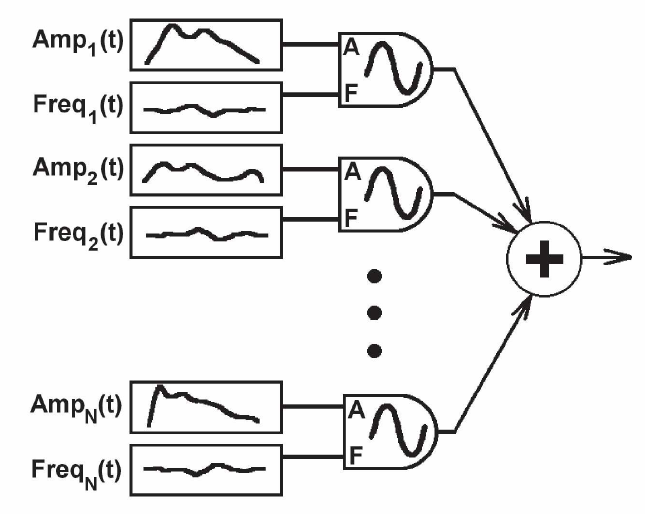
\includegraphics[width=0.5\textwidth]{sinusoidal_add_synth.PNG}
      \caption{Sinusoidal Additive Synthesis Algorithm \cite{Cook:2002:RSS:515316}.}
      \label{fig:sin_add_synth}
\end{figure}

Mathematically, at a struck point $k$ when vibrating in mode $n$, the impulse response of the model is:
\begin{equation}\label{eq:modal_response}
y_k = \sum\limits_{n=1}^{N} A_{nk}\ e^{-d_n t}\ \cos(2 \pi f_nt)
\end{equation}
if $t>=0$ and $y_k = 0$ if $t<0$ \cite{van2001foleyautomatic}.

\subsection{Filter-based Modal Synthesis}\label{sec:add_synth}

\paragraph{Band-pass Filters\\}\label{par:bpf}

At this point we will give some basic description of the band-pass filter since it is widely used in this thesis. Band-pass filters (BPFs) take a signal as input and give only a range of it as output, attenuating the rest of the frequencies. This range depends on the central frequency $f_c$. A filter of this kind is a result of a cascading of a low-pass and a high-pass filter circuit.

The passing range or ``band'' of frequencies is called \textbf{Bandwidth (BW)}. Defining as 0db the resonant peak, we can find the two cut-off frequencies ($f_{c{_\textsc{lower}}}$ and $f_{c_{\textsc{higher}}}$) at -3dB. The range between them is the bandwidth (equation \ref{eq:bw}). In figure \ref{fig:resp_bpf} we can see the frequency response of a BPF. \cite{bib:bpf}. 
\begin{equation}\label{eq:bw}
BW = f_{c_{\textsc{higher}}}-f_{c_{\textsc{lower}}}
\end{equation}   

\begin{figure}[H]
  \centering
    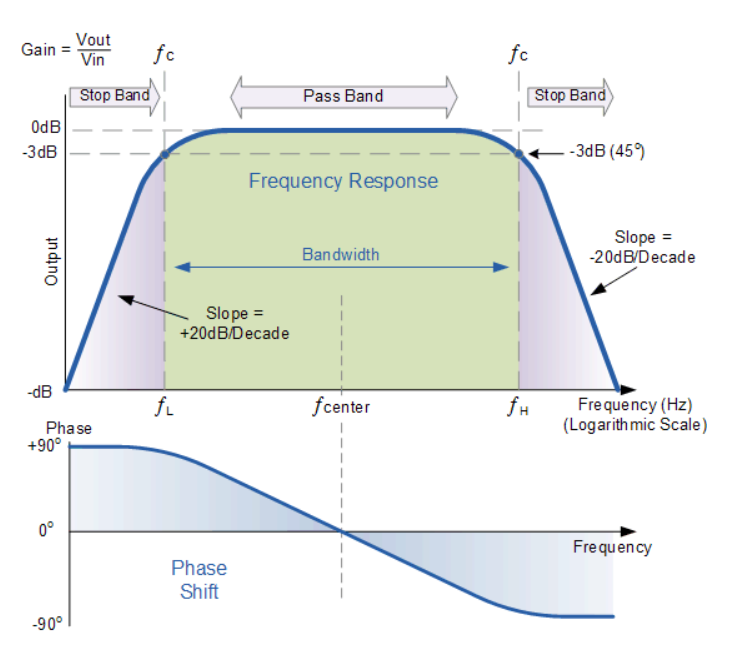
\includegraphics[width=0.7\textwidth]{BPF.PNG}
      \caption{Frequency Response of a Band-pass Filter  \cite{bib:bpf}.}
      \label{fig:resp_bpf}
\end{figure}

\paragraph{Synthesis\\}\label{par:synth}

This method is also additive, since we are adding the outputs of a number of band-pass filters. To synthesize a sound using this method, we use as many filters as the modal frequencies. The filter takes as input an impulse, the center frequency which is the modal frequency and a \textbf{Quality factor (Q-factor)} which specifies the bandwidth of the filter. The Q-factor is calculated heuristically, depending on the material of the sound and is inversely proportional to the bandwidth ($Q=f_c/BW$), so the lower the Q-factor, the wider the bandwidth and vice-versa. Hence, more or less frequencies will be included in the \colorbox{pink}{audible} range. We call the above structure a \textit{resonator}, which also includes a multiplication with the corresponding amplitude, taken from the $A$ matrix.

\begin{figure}[H]
  \centering
    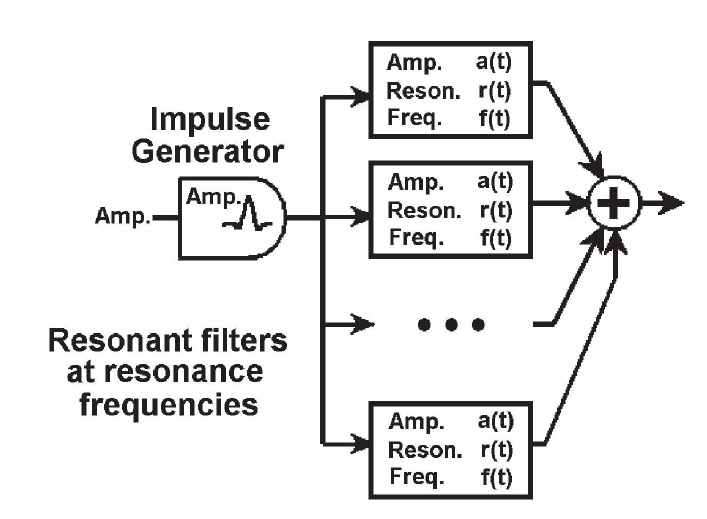
\includegraphics[width=0.5\textwidth]{filter-based_add_synth.PNG}
      \caption{Filter-based Modal Synthesis Algorithm \cite{Cook:2002:RSS:515316}.}
      \label{fig:filter_synth}
\end{figure}

\subsection{Sound Variations} \label{sec:sound_variation}
Each point of an object produces a different sound when struck. This happens because of the different amount of excitation each resonant mode experiences. As mentioned above, during data extraction we get a matrix of amplitudes of size $NxK$ corresponding to $K$ different resonant modes of each of the $N$ points of the object. This means that even though resonant frequencies are the same for each location of the specified object, each frequency's peak differentiated depending on the location.

There are several methods to achieve spatial variation on sound produced from the same object. 
\begin{enumerate}
\item The most accurate method is to perform FEM analysis on the object and distill as many amplitude matrices as the number of points consisting it. However, this method needs a lot of memory to store the data and computational power to access them.
\item Another less precise method is to separate the object into areas and compromise that each point belonging in the same area sound exactly the same. Thus, the amount of stored data decreases in a great deal when at the same time the sounding result is almost the same.
\item A third method is to store only one amplitude matrix and randomize the values for each impact sound, but this can lead to an unexpected behavior.
\item Finally, a better approach to the previous method is to retain the same amplitude values for all points of the object, but apply a texture map on the object which indicates changes on the pitch of the sound all over the object. For instance, the near-edge points of an object produce a higher-pitched sound than the ones in the center of each faces \cite{lloyd2011sound}. 
\end{enumerate}

\section{3D Audio}
In VR/AR applications, the location of the incoming sound plays as significant role as the sound itself. 

